\documentclass[1p]{elsarticle_modified}
%\bibliographystyle{elsarticle-num}

%\usepackage[colorlinks]{hyperref}
%\usepackage{abbrmath_seonhwa} %\Abb, \Ascr, \Acal ,\Abf, \Afrak
\usepackage{amsfonts}
\usepackage{amssymb}
\usepackage{amsmath}
\usepackage{amsthm}
\usepackage{scalefnt}
\usepackage{amsbsy}
\usepackage{kotex}
\usepackage{caption}
\usepackage{subfig}
\usepackage{color}
\usepackage{graphicx}
\usepackage{xcolor} %% white, black, red, green, blue, cyan, magenta, yellow
\usepackage{float}
\usepackage{setspace}
\usepackage{hyperref}

\usepackage{tikz}
\usetikzlibrary{arrows}

\usepackage{multirow}
\usepackage{array} % fixed length table
\usepackage{hhline}

%%%%%%%%%%%%%%%%%%%%%
\makeatletter
\renewcommand*\env@matrix[1][\arraystretch]{%
	\edef\arraystretch{#1}%
	\hskip -\arraycolsep
	\let\@ifnextchar\new@ifnextchar
	\array{*\c@MaxMatrixCols c}}
\makeatother %https://tex.stackexchange.com/questions/14071/how-can-i-increase-the-line-spacing-in-a-matrix
%%%%%%%%%%%%%%%

\usepackage[normalem]{ulem}

\newcommand{\msout}[1]{\ifmmode\text{\sout{\ensuremath{#1}}}\else\sout{#1}\fi}
%SOURCE: \msout is \stkout macro in https://tex.stackexchange.com/questions/20609/strikeout-in-math-mode

\newcommand{\cancel}[1]{
	\ifmmode
	{\color{red}\msout{#1}}
	\else
	{\color{red}\sout{#1}}
	\fi
}

\newcommand{\add}[1]{
	{\color{blue}\uwave{#1}}
}

\newcommand{\replace}[2]{
	\ifmmode
	{\color{red}\msout{#1}}{\color{blue}\uwave{#2}}
	\else
	{\color{red}\sout{#1}}{\color{blue}\uwave{#2}}
	\fi
}

\newcommand{\Sol}{\mathcal{S}} %segment
\newcommand{\D}{D} %diagram
\newcommand{\A}{\mathcal{A}} %arc


%%%%%%%%%%%%%%%%%%%%%%%%%%%%%5 test

\def\sl{\operatorname{\textup{SL}}(2,\Cbb)}
\def\psl{\operatorname{\textup{PSL}}(2,\Cbb)}
\def\quan{\mkern 1mu \triangleright \mkern 1mu}

\theoremstyle{definition}
\newtheorem{thm}{Theorem}[section]
\newtheorem{prop}[thm]{Proposition}
\newtheorem{lem}[thm]{Lemma}
\newtheorem{ques}[thm]{Question}
\newtheorem{cor}[thm]{Corollary}
\newtheorem{defn}[thm]{Definition}
\newtheorem{exam}[thm]{Example}
\newtheorem{rmk}[thm]{Remark}
\newtheorem{alg}[thm]{Algorithm}

\newcommand{\I}{\sqrt{-1}}
\begin{document}

%\begin{frontmatter}
%
%\title{Boundary parabolic representations of knots up to 8 crossings}
%
%%% Group authors per affiliation:
%\author{Yunhi Cho} 
%\address{Department of Mathematics, University of Seoul, Seoul, Korea}
%\ead{yhcho@uos.ac.kr}
%
%
%\author{Seonhwa Kim} %\fnref{s_kim}}
%\address{Center for Geometry and Physics, Institute for Basic Science, Pohang, 37673, Korea}
%\ead{ryeona17@ibs.re.kr}
%
%\author{Hyuk Kim}
%\address{Department of Mathematical Sciences, Seoul National University, Seoul 08826, Korea}
%\ead{hyukkim@snu.ac.kr}
%
%\author{Seokbeom Yoon}
%\address{Department of Mathematical Sciences, Seoul National University, Seoul, 08826,  Korea}
%\ead{sbyoon15@snu.ac.kr}
%
%\begin{abstract}
%We find all boundary parabolic representation of knots up to 8 crossings.
%
%\end{abstract}
%\begin{keyword}
%    \MSC[2010] 57M25 
%\end{keyword}
%
%\end{frontmatter}

%\linenumbers
%\tableofcontents
%
\newcommand\colored[1]{\textcolor{white}{\rule[-0.35ex]{0.8em}{1.4ex}}\kern-0.8em\color{red} #1}%
%\newcommand\colored[1]{\textcolor{white}{ #1}\kern-2.17ex	\textcolor{white}{ #1}\kern-1.81ex	\textcolor{white}{ #1}\kern-2.15ex\color{red}#1	}

{\Large $\underline{12n_{0336}~(K12n_{0336})}$}

\setlength{\tabcolsep}{10pt}
\renewcommand{\arraystretch}{1.6}
\vspace{1cm}\begin{tabular}{m{100pt}>{\centering\arraybackslash}m{274pt}}
\multirow{5}{120pt}{
	\centering
	\includegraphics[width=112pt]{../../../GIT/diagram.site/Diagrams/png/2425_12n_0336.png}\\
\ \ \ A knot diagram\footnotemark}&
\allowdisplaybreaks
\textbf{Linearized knot diagam} \\
\cline{2-2}
 &
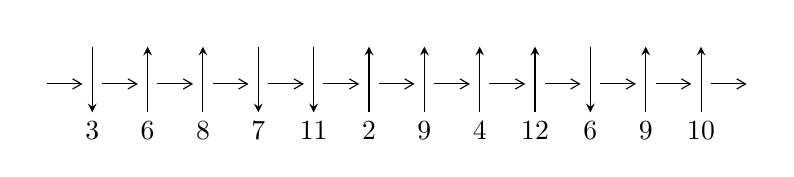
\begin{tikzpicture}[x=20pt, y=17pt]
	% nodes
	\node (C0) at (0, 0) {};
	\node (C1) at (1, 0) {};
	\node (C1U) at (1, +1) {};
	\node (C1D) at (1, -1) {3};

	\node (C2) at (2, 0) {};
	\node (C2U) at (2, +1) {};
	\node (C2D) at (2, -1) {6};

	\node (C3) at (3, 0) {};
	\node (C3U) at (3, +1) {};
	\node (C3D) at (3, -1) {8};

	\node (C4) at (4, 0) {};
	\node (C4U) at (4, +1) {};
	\node (C4D) at (4, -1) {7};

	\node (C5) at (5, 0) {};
	\node (C5U) at (5, +1) {};
	\node (C5D) at (5, -1) {11};

	\node (C6) at (6, 0) {};
	\node (C6U) at (6, +1) {};
	\node (C6D) at (6, -1) {2};

	\node (C7) at (7, 0) {};
	\node (C7U) at (7, +1) {};
	\node (C7D) at (7, -1) {9};

	\node (C8) at (8, 0) {};
	\node (C8U) at (8, +1) {};
	\node (C8D) at (8, -1) {4};

	\node (C9) at (9, 0) {};
	\node (C9U) at (9, +1) {};
	\node (C9D) at (9, -1) {12};

	\node (C10) at (10, 0) {};
	\node (C10U) at (10, +1) {};
	\node (C10D) at (10, -1) {6};

	\node (C11) at (11, 0) {};
	\node (C11U) at (11, +1) {};
	\node (C11D) at (11, -1) {9};

	\node (C12) at (12, 0) {};
	\node (C12U) at (12, +1) {};
	\node (C12D) at (12, -1) {10};
	\node (C13) at (13, 0) {};

	% arrows
	\draw[->,>={angle 60}]
	(C0) edge (C1) (C1) edge (C2) (C2) edge (C3) (C3) edge (C4) (C4) edge (C5) (C5) edge (C6) (C6) edge (C7) (C7) edge (C8) (C8) edge (C9) (C9) edge (C10) (C10) edge (C11) (C11) edge (C12) (C12) edge (C13) ;	\draw[->,>=stealth]
	(C1U) edge (C1D) (C2D) edge (C2U) (C3D) edge (C3U) (C4U) edge (C4D) (C5U) edge (C5D) (C6D) edge (C6U) (C7D) edge (C7U) (C8D) edge (C8U) (C9D) edge (C9U) (C10U) edge (C10D) (C11D) edge (C11U) (C12D) edge (C12U) ;
	\end{tikzpicture} \\
\hhline{~~} \\& 
\textbf{Solving Sequence} \\ \cline{2-2} 
 &
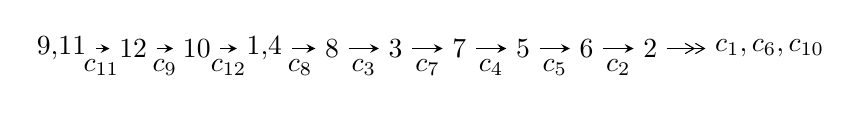
\begin{tikzpicture}[x=23pt, y=7pt]
	% node
	\node (A0) at (-1/8, 0) {9,11};
	\node (A1) at (1, 0) {12};
	\node (A2) at (2, 0) {10};
	\node (A3) at (49/16, 0) {1,4};
	\node (A4) at (33/8, 0) {8};
	\node (A5) at (41/8, 0) {3};
	\node (A6) at (49/8, 0) {7};
	\node (A7) at (57/8, 0) {5};
	\node (A8) at (65/8, 0) {6};
	\node (A9) at (73/8, 0) {2};
	\node (C1) at (1/2, -1) {$c_{11}$};
	\node (C2) at (3/2, -1) {$c_{9}$};
	\node (C3) at (5/2, -1) {$c_{12}$};
	\node (C4) at (29/8, -1) {$c_{8}$};
	\node (C5) at (37/8, -1) {$c_{3}$};
	\node (C6) at (45/8, -1) {$c_{7}$};
	\node (C7) at (53/8, -1) {$c_{4}$};
	\node (C8) at (61/8, -1) {$c_{5}$};
	\node (C9) at (69/8, -1) {$c_{2}$};
	\node (A10) at (11, 0) {$c_{1},c_{6},c_{10}$};

	% edge
	\draw[->,>=stealth]	
	(A0) edge (A1) (A1) edge (A2) (A2) edge (A3) (A3) edge (A4) (A4) edge (A5) (A5) edge (A6) (A6) edge (A7) (A7) edge (A8) (A8) edge (A9) ;
	\draw[->>,>={angle 60}]	
	(A9) edge (A10);
\end{tikzpicture} \\ 

\end{tabular} \\

\footnotetext{
The image of knot diagram is generated by the software ``\textbf{Draw programme}" developed by Andrew Bartholomew(\url{http://www.layer8.co.uk/maths/draw/index.htm\#Running-draw}), where we modified some parts for our purpose(\url{https://github.com/CATsTAILs/LinksPainter}).
}\phantom \\ \newline 
\centering \textbf{Ideals for irreducible components\footnotemark of $X_{\text{par}}$} 
 
\begin{align*}
I^u_{1}&=\langle 
-1706550177091 u^{18}-23512487300441 u^{17}+\cdots+39336273597696 b-69157159108721,\\
\phantom{I^u_{1}}&\phantom{= \langle  }-32608816754461 u^{18}-456051534293894 u^{17}+\cdots+19668136798848 a-1093408920959144,\\
\phantom{I^u_{1}}&\phantom{= \langle  }u^{19}+14 u^{18}+\cdots+52 u+1\rangle \\
I^u_{2}&=\langle 
- a^8+a^7+3 a^6-2 a^5-3 a^4+2 a^3+b+a+2,\;a^9- a^8-2 a^7+3 a^6+a^5-3 a^4+2 a^3- a+1,\;u-1\rangle \\
I^u_{3}&=\langle 
-3 a^3 u+2 a^3- a^2 u+b+a,\;a^4- a^2 u-2 a^2+3 u+5,\;u^2+u-1\rangle \\
\\
\end{align*}
\raggedright * 3 irreducible components of $\dim_{\mathbb{C}}=0$, with total 36 representations.\\
\footnotetext{All coefficients of polynomials are rational numbers. But the coefficients are sometimes approximated in decimal forms when there is not enough margin.}
\newpage
\renewcommand{\arraystretch}{1}
\centering \section*{I. $I^u_{1}= \langle -1.71\times10^{12} u^{18}-2.35\times10^{13} u^{17}+\cdots+3.93\times10^{13} b-6.92\times10^{13},\;-3.26\times10^{13} u^{18}-4.56\times10^{14} u^{17}+\cdots+1.97\times10^{13} a-1.09\times10^{15},\;u^{19}+14 u^{18}+\cdots+52 u+1 \rangle$}
\flushleft \textbf{(i) Arc colorings}\\
\begin{tabular}{m{7pt} m{180pt} m{7pt} m{180pt} }
\flushright $a_{9}=$&$\begin{pmatrix}0\\u\end{pmatrix}$ \\
\flushright $a_{11}=$&$\begin{pmatrix}1\\0\end{pmatrix}$ \\
\flushright $a_{12}=$&$\begin{pmatrix}1\\- u^2\end{pmatrix}$ \\
\flushright $a_{10}=$&$\begin{pmatrix}u\\- u^3+u\end{pmatrix}$ \\
\flushright $a_{1}=$&$\begin{pmatrix}- u^2+1\\u^4-2 u^2\end{pmatrix}$ \\
\flushright $a_{4}=$&$\begin{pmatrix}1.65795 u^{18}+23.1873 u^{17}+\cdots+1589.07 u+55.5929\\0.0433836 u^{18}+0.597730 u^{17}+\cdots+39.8060 u+1.75810\end{pmatrix}$ \\
\flushright $a_{8}=$&$\begin{pmatrix}1.84251 u^{18}+25.7334 u^{17}+\cdots+1669.72 u+43.2886\\0.0542335 u^{18}+0.767279 u^{17}+\cdots+55.0156 u+1.70577\end{pmatrix}$ \\
\flushright $a_{3}=$&$\begin{pmatrix}0.243745 u^{18}+3.43967 u^{17}+\cdots+332.641 u+35.7067\\-0.0193717 u^{18}-0.267431 u^{17}+\cdots-10.7266 u+0.631068\end{pmatrix}$ \\
\flushright $a_{7}=$&$\begin{pmatrix}1.84251 u^{18}+25.7334 u^{17}+\cdots+1669.72 u+43.2886\\0.0598519 u^{18}+0.839590 u^{17}+\cdots+56.3822 u+1.76749\end{pmatrix}$ \\
\flushright $a_{5}=$&$\begin{pmatrix}0.0513825 u^{18}+0.731152 u^{17}+\cdots+83.7307 u+7.87385\\-0.00184480 u^{18}-0.0331746 u^{17}+\cdots-3.98487 u+0.0723727\end{pmatrix}$ \\
\flushright $a_{6}=$&$\begin{pmatrix}0.0532273 u^{18}+0.764327 u^{17}+\cdots+87.7156 u+7.80147\\-0.00184480 u^{18}-0.0331746 u^{17}+\cdots-3.98487 u+0.0723727\end{pmatrix}$ \\
\flushright $a_{2}=$&$\begin{pmatrix}-0.136733 u^{18}-1.87566 u^{17}+\cdots-19.9103 u+26.8869\\-0.0281326 u^{18}-0.392506 u^{17}+\cdots-21.4809 u+0.261960\end{pmatrix}$\\&\end{tabular}
\flushleft \textbf{(ii) Obstruction class $= -1$}\\~\\
\flushleft \textbf{(iii) Cusp Shapes $= -\frac{390713901803}{1639011399904} u^{18}-\frac{21917006139285}{6556045599616} u^{17}+\cdots-\frac{430703611764529}{1639011399904} u-\frac{74684759366323}{6556045599616}$}\\~\\
\newpage\renewcommand{\arraystretch}{1}
\flushleft \textbf{(iv) u-Polynomials at the component}\newline \\
\begin{tabular}{m{50pt}|m{274pt}}
Crossings & \hspace{64pt}u-Polynomials at each crossing \\
\hline $$\begin{aligned}c_{1}\end{aligned}$$&$\begin{aligned}
&u^{19}-9 u^{18}+\cdots+9432 u-1296
\end{aligned}$\\
\hline $$\begin{aligned}c_{2},c_{6}\end{aligned}$$&$\begin{aligned}
&u^{19}-7 u^{18}+\cdots-36 u+36
\end{aligned}$\\
\hline $$\begin{aligned}c_{3},c_{8}\end{aligned}$$&$\begin{aligned}
&u^{19}-2 u^{18}+\cdots-12 u+9
\end{aligned}$\\
\hline $$\begin{aligned}c_{4}\end{aligned}$$&$\begin{aligned}
&u^{19}-6 u^{18}+\cdots+19710 u-2349
\end{aligned}$\\
\hline $$\begin{aligned}c_{5},c_{10}\end{aligned}$$&$\begin{aligned}
&u^{19}+u^{18}+\cdots+1536 u+512
\end{aligned}$\\
\hline $$\begin{aligned}c_{7}\end{aligned}$$&$\begin{aligned}
&u^{19}-16 u^{18}+\cdots+540 u-81
\end{aligned}$\\
\hline $$\begin{aligned}c_{9},c_{11},c_{12}\end{aligned}$$&$\begin{aligned}
&u^{19}+14 u^{18}+\cdots+52 u+1
\end{aligned}$\\
\hline
\end{tabular}\\~\\
\newpage\renewcommand{\arraystretch}{1}
\flushleft \textbf{(v) Riley Polynomials at the component}\newline \\
\begin{tabular}{m{50pt}|m{274pt}}
Crossings & \hspace{64pt}Riley Polynomials at each crossing \\
\hline $$\begin{aligned}c_{1}\end{aligned}$$&$\begin{aligned}
&y^{19}- y^{18}+\cdots+159068448 y-1679616
\end{aligned}$\\
\hline $$\begin{aligned}c_{2},c_{6}\end{aligned}$$&$\begin{aligned}
&y^{19}-9 y^{18}+\cdots+9432 y-1296
\end{aligned}$\\
\hline $$\begin{aligned}c_{3},c_{8}\end{aligned}$$&$\begin{aligned}
&y^{19}-16 y^{18}+\cdots+540 y-81
\end{aligned}$\\
\hline $$\begin{aligned}c_{4}\end{aligned}$$&$\begin{aligned}
&y^{19}+56 y^{18}+\cdots+419265396 y-5517801
\end{aligned}$\\
\hline $$\begin{aligned}c_{5},c_{10}\end{aligned}$$&$\begin{aligned}
&y^{19}+69 y^{18}+\cdots+15204352 y-262144
\end{aligned}$\\
\hline $$\begin{aligned}c_{7}\end{aligned}$$&$\begin{aligned}
&y^{19}-20 y^{18}+\cdots+220968 y-6561
\end{aligned}$\\
\hline $$\begin{aligned}c_{9},c_{11},c_{12}\end{aligned}$$&$\begin{aligned}
&y^{19}-72 y^{18}+\cdots+696 y-1
\end{aligned}$\\
\hline
\end{tabular}\\~\\
\newpage\flushleft \textbf{(vi) Complex Volumes and Cusp Shapes}
$$\begin{array}{c|c|c}  
\text{Solutions to }I^u_{1}& \I (\text{vol} + \sqrt{-1}CS) & \text{Cusp shape}\\
 \hline 
\begin{aligned}
u &= \phantom{-}1.090810 + 0.087492 I \\
a &= \phantom{-}0.864947 + 0.453435 I \\
b &= \phantom{-}1.25966 - 4.27188 I\end{aligned}
 & \phantom{-}0.12746 + 2.07953 I & \phantom{-}0.79710 + 6.78619 I \\ \hline\begin{aligned}
u &= \phantom{-}1.090810 - 0.087492 I \\
a &= \phantom{-}0.864947 - 0.453435 I \\
b &= \phantom{-}1.25966 + 4.27188 I\end{aligned}
 & \phantom{-}0.12746 - 2.07953 I & \phantom{-}0.79710 - 6.78619 I \\ \hline\begin{aligned}
u &= \phantom{-}1.12421\phantom{ +0.000000I} \\
a &= -0.369206\phantom{ +0.000000I} \\
b &= -0.262337\phantom{ +0.000000I}\end{aligned}
 & \phantom{-}2.16627\phantom{ +0.000000I} & \phantom{-}2.38650\phantom{ +0.000000I} \\ \hline\begin{aligned}
u &= -0.866404 + 0.903603 I \\
a &= \phantom{-}0.403452 + 1.041090 I \\
b &= -1.260210 - 0.033364 I\end{aligned}
 & \phantom{-}4.84224 + 5.75329 I & \phantom{-}6.23581 - 2.60069 I \\ \hline\begin{aligned}
u &= -0.866404 - 0.903603 I \\
a &= \phantom{-}0.403452 - 1.041090 I \\
b &= -1.260210 + 0.033364 I\end{aligned}
 & \phantom{-}4.84224 - 5.75329 I & \phantom{-}6.23581 + 2.60069 I \\ \hline\begin{aligned}
u &= \phantom{-}0.264112 + 0.511238 I \\
a &= \phantom{-}0.998671 + 0.095546 I \\
b &= \phantom{-}0.655201 - 0.830329 I\end{aligned}
 & \phantom{-}0.335625 + 1.223470 I & \phantom{-}4.13138 - 4.81848 I \\ \hline\begin{aligned}
u &= \phantom{-}0.264112 - 0.511238 I \\
a &= \phantom{-}0.998671 - 0.095546 I \\
b &= \phantom{-}0.655201 + 0.830329 I\end{aligned}
 & \phantom{-}0.335625 - 1.223470 I & \phantom{-}4.13138 + 4.81848 I \\ \hline\begin{aligned}
u &= -1.54015 + 0.03306 I \\
a &= -0.616311 + 0.224492 I \\
b &= \phantom{-}0.39526 - 1.71073 I\end{aligned}
 & \phantom{-}8.24788 - 1.49342 I & \phantom{-}14.3201 - 0.4966 I \\ \hline\begin{aligned}
u &= -1.54015 - 0.03306 I \\
a &= -0.616311 - 0.224492 I \\
b &= \phantom{-}0.39526 + 1.71073 I\end{aligned}
 & \phantom{-}8.24788 + 1.49342 I & \phantom{-}14.3201 + 0.4966 I \\ \hline\begin{aligned}
u &= -0.272498\phantom{ +0.000000I} \\
a &= -3.42293\phantom{ +0.000000I} \\
b &= -0.561462\phantom{ +0.000000I}\end{aligned}
 & \phantom{-}1.52167\phantom{ +0.000000I} & \phantom{-}5.90680\phantom{ +0.000000I}\\
 \hline 
 \end{array}$$\newpage$$\begin{array}{c|c|c}  
\text{Solutions to }I^u_{1}& \I (\text{vol} + \sqrt{-1}CS) & \text{Cusp shape}\\
 \hline 
\begin{aligned}
u &= -0.0292040 + 0.0188465 I \\
a &= \phantom{-}11.6667 + 24.4338 I \\
b &= \phantom{-}0.653657 + 0.621796 I\end{aligned}
 & -1.74489 + 2.05954 I & -4.07768 - 4.15264 I \\ \hline\begin{aligned}
u &= -0.0292040 - 0.0188465 I \\
a &= \phantom{-}11.6667 - 24.4338 I \\
b &= \phantom{-}0.653657 - 0.621796 I\end{aligned}
 & -1.74489 - 2.05954 I & -4.07768 + 4.15264 I \\ \hline\begin{aligned}
u &= -2.00138 + 0.76457 I \\
a &= -0.689796 + 0.112485 I \\
b &= -0.56693 - 3.57760 I\end{aligned}
 & -15.5608 - 12.7812 I & \phantom{-}6.72063 + 5.11794 I \\ \hline\begin{aligned}
u &= -2.00138 - 0.76457 I \\
a &= -0.689796 - 0.112485 I \\
b &= -0.56693 + 3.57760 I\end{aligned}
 & -15.5608 + 12.7812 I & \phantom{-}6.72063 - 5.11794 I \\ \hline\begin{aligned}
u &= -2.42283 + 0.72006 I \\
a &= \phantom{-}0.017324 - 0.538247 I \\
b &= \phantom{-}2.30004 + 3.34538 I\end{aligned}
 & -18.5440 - 5.6494 I & \phantom{-}4.00000 + 0. I\phantom{ +0.000000I} \\ \hline\begin{aligned}
u &= -2.42283 - 0.72006 I \\
a &= \phantom{-}0.017324 + 0.538247 I \\
b &= \phantom{-}2.30004 - 3.34538 I\end{aligned}
 & -18.5440 + 5.6494 I & \phantom{-}4.00000 + 0. I\phantom{ +0.000000I} \\ \hline\begin{aligned}
u &= -3.92517 + 0.42402 I \\
a &= \phantom{-}0.495462 - 0.122568 I \\
b &= -4.38040 + 4.23334 I\end{aligned}
 & -11.60890 - 1.83503 I & \phantom{-0.000000 } 0 \\ \hline\begin{aligned}
u &= -3.92517 - 0.42402 I \\
a &= \phantom{-}0.495462 + 0.122568 I \\
b &= -4.38040 - 4.23334 I\end{aligned}
 & -11.60890 + 1.83503 I & \phantom{-0.000000 } 0 \\ \hline\begin{aligned}
u &= \phantom{-}4.00873\phantom{ +0.000000I} \\
a &= \phantom{-}0.511273\phantom{ +0.000000I} \\
b &= -5.28877\phantom{ +0.000000I}\end{aligned}
 & \phantom{-}11.4850\phantom{ +0.000000I} & \phantom{-0.000000 } 0\\
 \hline 
 \end{array}$$\newpage\newpage\renewcommand{\arraystretch}{1}
\centering \section*{II. $I^u_{2}= \langle - a^8+a^7+3 a^6-2 a^5-3 a^4+2 a^3+b+a+2,\;a^9- a^8-2 a^7+3 a^6+a^5-3 a^4+2 a^3- a+1,\;u-1 \rangle$}
\flushleft \textbf{(i) Arc colorings}\\
\begin{tabular}{m{7pt} m{180pt} m{7pt} m{180pt} }
\flushright $a_{9}=$&$\begin{pmatrix}0\\1\end{pmatrix}$ \\
\flushright $a_{11}=$&$\begin{pmatrix}1\\0\end{pmatrix}$ \\
\flushright $a_{12}=$&$\begin{pmatrix}1\\-1\end{pmatrix}$ \\
\flushright $a_{10}=$&$\begin{pmatrix}1\\0\end{pmatrix}$ \\
\flushright $a_{1}=$&$\begin{pmatrix}0\\-1\end{pmatrix}$ \\
\flushright $a_{4}=$&$\begin{pmatrix}a\\a^8- a^7-3 a^6+2 a^5+3 a^4-2 a^3- a-2\end{pmatrix}$ \\
\flushright $a_{8}=$&$\begin{pmatrix}- a^2\\a^7+a^6-2 a^5- a^4+2 a^3+a^2+a+2\end{pmatrix}$ \\
\flushright $a_{3}=$&$\begin{pmatrix}- a^3+a\\2 a^8-5 a^6+a^5+5 a^4- a^3+a^2+a-2\end{pmatrix}$ \\
\flushright $a_{7}=$&$\begin{pmatrix}- a^2\\a^7+a^6-2 a^5- a^4+2 a^3+a+2\end{pmatrix}$ \\
\flushright $a_{5}=$&$\begin{pmatrix}a^5- a^3+a\\0\end{pmatrix}$ \\
\flushright $a_{6}=$&$\begin{pmatrix}a^5- a^3+a\\0\end{pmatrix}$ \\
\flushright $a_{2}=$&$\begin{pmatrix}a^6-2 a^4+a^2\\2 a^8-5 a^6+a^5+5 a^4- a^3+a^2+a-2\end{pmatrix}$\\&\end{tabular}
\flushleft \textbf{(ii) Obstruction class $= 1$}\\~\\
\flushleft \textbf{(iii) Cusp Shapes $= 6 a^8-3 a^7-10 a^6+8 a^5+2 a^4-8 a^3+12 a^2+6$}\\~\\
\newpage\renewcommand{\arraystretch}{1}
\flushleft \textbf{(iv) u-Polynomials at the component}\newline \\
\begin{tabular}{m{50pt}|m{274pt}}
Crossings & \hspace{64pt}u-Polynomials at each crossing \\
\hline $$\begin{aligned}c_{1},c_{4}\end{aligned}$$&$\begin{aligned}
&u^9-3 u^8+8 u^7-13 u^6+17 u^5-17 u^4+12 u^3-6 u^2+u+1
\end{aligned}$\\
\hline $$\begin{aligned}c_{2}\end{aligned}$$&$\begin{aligned}
&u^9- u^8+2 u^7- u^6+3 u^5- u^4+2 u^3+u+1
\end{aligned}$\\
\hline $$\begin{aligned}c_{3}\end{aligned}$$&$\begin{aligned}
&u^9- u^8-2 u^7+3 u^6+u^5-3 u^4+2 u^3- u+1
\end{aligned}$\\
\hline $$\begin{aligned}c_{5},c_{10}\end{aligned}$$&$\begin{aligned}
&u^9
\end{aligned}$\\
\hline $$\begin{aligned}c_{6}\end{aligned}$$&$\begin{aligned}
&u^9+u^8+2 u^7+u^6+3 u^5+u^4+2 u^3+u-1
\end{aligned}$\\
\hline $$\begin{aligned}c_{7}\end{aligned}$$&$\begin{aligned}
&u^9+5 u^8+12 u^7+15 u^6+9 u^5- u^4-4 u^3-2 u^2+u+1
\end{aligned}$\\
\hline $$\begin{aligned}c_{8}\end{aligned}$$&$\begin{aligned}
&u^9+u^8-2 u^7-3 u^6+u^5+3 u^4+2 u^3- u-1
\end{aligned}$\\
\hline $$\begin{aligned}c_{9}\end{aligned}$$&$\begin{aligned}
&(u+1)^9
\end{aligned}$\\
\hline $$\begin{aligned}c_{11},c_{12}\end{aligned}$$&$\begin{aligned}
&(u-1)^9
\end{aligned}$\\
\hline
\end{tabular}\\~\\
\newpage\renewcommand{\arraystretch}{1}
\flushleft \textbf{(v) Riley Polynomials at the component}\newline \\
\begin{tabular}{m{50pt}|m{274pt}}
Crossings & \hspace{64pt}Riley Polynomials at each crossing \\
\hline $$\begin{aligned}c_{1},c_{4}\end{aligned}$$&$\begin{aligned}
&y^9+7 y^8+20 y^7+25 y^6+5 y^5-15 y^4+22 y^2+13 y-1
\end{aligned}$\\
\hline $$\begin{aligned}c_{2},c_{6}\end{aligned}$$&$\begin{aligned}
&y^9+3 y^8+8 y^7+13 y^6+17 y^5+17 y^4+12 y^3+6 y^2+y-1
\end{aligned}$\\
\hline $$\begin{aligned}c_{3},c_{8}\end{aligned}$$&$\begin{aligned}
&y^9-5 y^8+12 y^7-15 y^6+9 y^5+y^4-4 y^3+2 y^2+y-1
\end{aligned}$\\
\hline $$\begin{aligned}c_{5},c_{10}\end{aligned}$$&$\begin{aligned}
&y^9
\end{aligned}$\\
\hline $$\begin{aligned}c_{7}\end{aligned}$$&$\begin{aligned}
&y^9- y^8+12 y^7-7 y^6+37 y^5+y^4-10 y^2+5 y-1
\end{aligned}$\\
\hline $$\begin{aligned}c_{9},c_{11},c_{12}\end{aligned}$$&$\begin{aligned}
&(y-1)^9
\end{aligned}$\\
\hline
\end{tabular}\\~\\
\newpage\flushleft \textbf{(vi) Complex Volumes and Cusp Shapes}
$$\begin{array}{c|c|c}  
\text{Solutions to }I^u_{2}& \I (\text{vol} + \sqrt{-1}CS) & \text{Cusp shape}\\
 \hline 
\begin{aligned}
u &= \phantom{-}1.00000\phantom{ +0.000000I} \\
a &= \phantom{-}0.772920 + 0.510351 I \\
b &= -3.25219 + 0.42284 I\end{aligned}
 & -0.13850 + 2.09337 I & \phantom{-}11.64247 + 5.88316 I \\ \hline\begin{aligned}
u &= \phantom{-}1.00000\phantom{ +0.000000I} \\
a &= \phantom{-}0.772920 - 0.510351 I \\
b &= -3.25219 - 0.42284 I\end{aligned}
 & -0.13850 - 2.09337 I & \phantom{-}11.64247 - 5.88316 I \\ \hline\begin{aligned}
u &= \phantom{-}1.00000\phantom{ +0.000000I} \\
a &= -0.825933\phantom{ +0.000000I} \\
b &= \phantom{-}0.106533\phantom{ +0.000000I}\end{aligned}
 & \phantom{-}2.84338\phantom{ +0.000000I} & \phantom{-}15.4610\phantom{ +0.000000I} \\ \hline\begin{aligned}
u &= \phantom{-}1.00000\phantom{ +0.000000I} \\
a &= -1.173910 + 0.391555 I \\
b &= -0.121911 - 0.782086 I\end{aligned}
 & \phantom{-}6.01628 - 1.33617 I & \phantom{-}7.94914 + 0.75351 I \\ \hline\begin{aligned}
u &= \phantom{-}1.00000\phantom{ +0.000000I} \\
a &= -1.173910 - 0.391555 I \\
b &= -0.121911 + 0.782086 I\end{aligned}
 & \phantom{-}6.01628 + 1.33617 I & \phantom{-}7.94914 - 0.75351 I \\ \hline\begin{aligned}
u &= \phantom{-}1.00000\phantom{ +0.000000I} \\
a &= \phantom{-}0.141484 + 0.739668 I \\
b &= -0.217279 - 0.962736 I\end{aligned}
 & \phantom{-}2.26187 - 2.45442 I & \phantom{-}4.75622 + 3.91612 I \\ \hline\begin{aligned}
u &= \phantom{-}1.00000\phantom{ +0.000000I} \\
a &= \phantom{-}0.141484 - 0.739668 I \\
b &= -0.217279 + 0.962736 I\end{aligned}
 & \phantom{-}2.26187 + 2.45442 I & \phantom{-}4.75622 - 3.91612 I \\ \hline\begin{aligned}
u &= \phantom{-}1.00000\phantom{ +0.000000I} \\
a &= \phantom{-}1.172470 + 0.500383 I \\
b &= \phantom{-}0.038112 - 1.195250 I\end{aligned}
 & \phantom{-}5.24306 + 7.08493 I & \phantom{-}7.92182 - 8.89461 I \\ \hline\begin{aligned}
u &= \phantom{-}1.00000\phantom{ +0.000000I} \\
a &= \phantom{-}1.172470 - 0.500383 I \\
b &= \phantom{-}0.038112 + 1.195250 I\end{aligned}
 & \phantom{-}5.24306 - 7.08493 I & \phantom{-}7.92182 + 8.89461 I\\
 \hline 
 \end{array}$$\newpage\newpage\renewcommand{\arraystretch}{1}
\centering \section*{III. $I^u_{3}= \langle -3 a^3 u+2 a^3- a^2 u+b+a,\;a^4- a^2 u-2 a^2+3 u+5,\;u^2+u-1 \rangle$}
\flushleft \textbf{(i) Arc colorings}\\
\begin{tabular}{m{7pt} m{180pt} m{7pt} m{180pt} }
\flushright $a_{9}=$&$\begin{pmatrix}0\\u\end{pmatrix}$ \\
\flushright $a_{11}=$&$\begin{pmatrix}1\\0\end{pmatrix}$ \\
\flushright $a_{12}=$&$\begin{pmatrix}1\\u-1\end{pmatrix}$ \\
\flushright $a_{10}=$&$\begin{pmatrix}u\\- u+1\end{pmatrix}$ \\
\flushright $a_{1}=$&$\begin{pmatrix}u\\- u\end{pmatrix}$ \\
\flushright $a_{4}=$&$\begin{pmatrix}a\\3 a^3 u-2 a^3+a^2 u- a\end{pmatrix}$ \\
\flushright $a_{8}=$&$\begin{pmatrix}- a^2 u\\a^3 u- a^3+3 a^2 u- a^2\end{pmatrix}$ \\
\flushright $a_{3}=$&$\begin{pmatrix}a^3 u- a^3+a\\- a^3 u+a^3- a+u+1\end{pmatrix}$ \\
\flushright $a_{7}=$&$\begin{pmatrix}- a^2 u\\a^3 u- a^3+a^2 u\end{pmatrix}$ \\
\flushright $a_{5}=$&$\begin{pmatrix}0\\3 a^3 u-2 a^3\end{pmatrix}$ \\
\flushright $a_{6}=$&$\begin{pmatrix}-3 a^3 u+2 a^3\\3 a^3 u-2 a^3\end{pmatrix}$ \\
\flushright $a_{2}=$&$\begin{pmatrix}a^3 u- a^3+a+u\\- a^3 u+a^3- a+1\end{pmatrix}$\\&\end{tabular}
\flushleft \textbf{(ii) Obstruction class $= 1$}\\~\\
\flushleft \textbf{(iii) Cusp Shapes $= 4 a^2 u-4 a^2+8$}\\~\\
\newpage\renewcommand{\arraystretch}{1}
\flushleft \textbf{(iv) u-Polynomials at the component}\newline \\
\begin{tabular}{m{50pt}|m{274pt}}
Crossings & \hspace{64pt}u-Polynomials at each crossing \\
\hline $$\begin{aligned}c_{1}\end{aligned}$$&$\begin{aligned}
&(u-1)^8
\end{aligned}$\\
\hline $$\begin{aligned}c_{2},c_{6}\end{aligned}$$&$\begin{aligned}
&(u^2+1)^4
\end{aligned}$\\
\hline $$\begin{aligned}c_{3},c_{4},c_{8}\end{aligned}$$&$\begin{aligned}
&(u^4- u^2+1)^2
\end{aligned}$\\
\hline $$\begin{aligned}c_{5},c_{10}\end{aligned}$$&$\begin{aligned}
&(u^4+3 u^2+1)^2
\end{aligned}$\\
\hline $$\begin{aligned}c_{7}\end{aligned}$$&$\begin{aligned}
&(u^2+u+1)^4
\end{aligned}$\\
\hline $$\begin{aligned}c_{9}\end{aligned}$$&$\begin{aligned}
&(u^2- u-1)^4
\end{aligned}$\\
\hline $$\begin{aligned}c_{11},c_{12}\end{aligned}$$&$\begin{aligned}
&(u^2+u-1)^4
\end{aligned}$\\
\hline
\end{tabular}\\~\\
\newpage\renewcommand{\arraystretch}{1}
\flushleft \textbf{(v) Riley Polynomials at the component}\newline \\
\begin{tabular}{m{50pt}|m{274pt}}
Crossings & \hspace{64pt}Riley Polynomials at each crossing \\
\hline $$\begin{aligned}c_{1}\end{aligned}$$&$\begin{aligned}
&(y-1)^8
\end{aligned}$\\
\hline $$\begin{aligned}c_{2},c_{6}\end{aligned}$$&$\begin{aligned}
&(y+1)^8
\end{aligned}$\\
\hline $$\begin{aligned}c_{3},c_{4},c_{8}\end{aligned}$$&$\begin{aligned}
&(y^2- y+1)^4
\end{aligned}$\\
\hline $$\begin{aligned}c_{5},c_{10}\end{aligned}$$&$\begin{aligned}
&(y^2+3 y+1)^4
\end{aligned}$\\
\hline $$\begin{aligned}c_{7}\end{aligned}$$&$\begin{aligned}
&(y^2+y+1)^4
\end{aligned}$\\
\hline $$\begin{aligned}c_{9},c_{11},c_{12}\end{aligned}$$&$\begin{aligned}
&(y^2-3 y+1)^4
\end{aligned}$\\
\hline
\end{tabular}\\~\\
\newpage\flushleft \textbf{(vi) Complex Volumes and Cusp Shapes}
$$\begin{array}{c|c|c}  
\text{Solutions to }I^u_{3}& \I (\text{vol} + \sqrt{-1}CS) & \text{Cusp shape}\\
 \hline 
\begin{aligned}
u &= \phantom{-}0.618034\phantom{ +0.000000I} \\
a &= \phantom{-}1.40126 + 0.80902 I \\
b &= -0.592242 - 0.025792 I\end{aligned}
 & -0.65797 + 2.02988 I & \phantom{-}6.00000 - 3.46410 I \\ \hline\begin{aligned}
u &= \phantom{-}0.618034\phantom{ +0.000000I} \\
a &= \phantom{-}1.40126 - 0.80902 I \\
b &= -0.592242 + 0.025792 I\end{aligned}
 & -0.65797 - 2.02988 I & \phantom{-}6.00000 + 3.46410 I \\ \hline\begin{aligned}
u &= \phantom{-}0.618034\phantom{ +0.000000I} \\
a &= -1.40126 + 0.80902 I \\
b &= \phantom{-}2.21028 - 2.82831 I\end{aligned}
 & -0.65797 - 2.02988 I & \phantom{-}6.00000 + 3.46410 I \\ \hline\begin{aligned}
u &= \phantom{-}0.618034\phantom{ +0.000000I} \\
a &= -1.40126 - 0.80902 I \\
b &= \phantom{-}2.21028 + 2.82831 I\end{aligned}
 & -0.65797 + 2.02988 I & \phantom{-}6.00000 - 3.46410 I \\ \hline\begin{aligned}
u &= -1.61803\phantom{ +0.000000I} \\
a &= -0.535233 + 0.309017 I \\
b &= \phantom{-}0.226216 - 1.391820 I\end{aligned}
 & \phantom{-}7.23771 + 2.02988 I & \phantom{-}6.00000 - 3.46410 I \\ \hline\begin{aligned}
u &= -1.61803\phantom{ +0.000000I} \\
a &= -0.535233 - 0.309017 I \\
b &= \phantom{-}0.226216 + 1.391820 I\end{aligned}
 & \phantom{-}7.23771 - 2.02988 I & \phantom{-}6.00000 + 3.46410 I \\ \hline\begin{aligned}
u &= -1.61803\phantom{ +0.000000I} \\
a &= \phantom{-}0.535233 + 0.309017 I \\
b &= -0.84425 - 2.46228 I\end{aligned}
 & \phantom{-}7.23771 - 2.02988 I & \phantom{-}6.00000 + 3.46410 I \\ \hline\begin{aligned}
u &= -1.61803\phantom{ +0.000000I} \\
a &= \phantom{-}0.535233 - 0.309017 I \\
b &= -0.84425 + 2.46228 I\end{aligned}
 & \phantom{-}7.23771 + 2.02988 I & \phantom{-}6.00000 - 3.46410 I\\
 \hline 
 \end{array}$$\newpage
\newpage\renewcommand{\arraystretch}{1}
\centering \section*{ IV. u-Polynomials}
\begin{tabular}{m{50pt}|m{274pt}}
Crossings & \hspace{64pt}u-Polynomials at each crossing \\
\hline $$\begin{aligned}c_{1}\end{aligned}$$&$\begin{aligned}
&((u-1)^8)(u^9-3 u^8+\cdots+u+1)\\
&\cdot(u^{19}-9 u^{18}+\cdots+9432 u-1296)
\end{aligned}$\\
\hline $$\begin{aligned}c_{2}\end{aligned}$$&$\begin{aligned}
&(u^2+1)^4(u^9- u^8+2 u^7- u^6+3 u^5- u^4+2 u^3+u+1)\\
&\cdot(u^{19}-7 u^{18}+\cdots-36 u+36)
\end{aligned}$\\
\hline $$\begin{aligned}c_{3}\end{aligned}$$&$\begin{aligned}
&(u^4- u^2+1)^2(u^9- u^8-2 u^7+3 u^6+u^5-3 u^4+2 u^3- u+1)\\
&\cdot(u^{19}-2 u^{18}+\cdots-12 u+9)
\end{aligned}$\\
\hline $$\begin{aligned}c_{4}\end{aligned}$$&$\begin{aligned}
&(u^4- u^2+1)^2\\
&\cdot(u^9-3 u^8+8 u^7-13 u^6+17 u^5-17 u^4+12 u^3-6 u^2+u+1)\\
&\cdot(u^{19}-6 u^{18}+\cdots+19710 u-2349)
\end{aligned}$\\
\hline $$\begin{aligned}c_{5},c_{10}\end{aligned}$$&$\begin{aligned}
&u^9(u^4+3 u^2+1)^2(u^{19}+u^{18}+\cdots+1536 u+512)
\end{aligned}$\\
\hline $$\begin{aligned}c_{6}\end{aligned}$$&$\begin{aligned}
&(u^2+1)^4(u^9+u^8+2 u^7+u^6+3 u^5+u^4+2 u^3+u-1)\\
&\cdot(u^{19}-7 u^{18}+\cdots-36 u+36)
\end{aligned}$\\
\hline $$\begin{aligned}c_{7}\end{aligned}$$&$\begin{aligned}
&((u^2+u+1)^4)(u^9+5 u^8+\cdots+u+1)\\
&\cdot(u^{19}-16 u^{18}+\cdots+540 u-81)
\end{aligned}$\\
\hline $$\begin{aligned}c_{8}\end{aligned}$$&$\begin{aligned}
&(u^4- u^2+1)^2(u^9+u^8-2 u^7-3 u^6+u^5+3 u^4+2 u^3- u-1)\\
&\cdot(u^{19}-2 u^{18}+\cdots-12 u+9)
\end{aligned}$\\
\hline $$\begin{aligned}c_{9}\end{aligned}$$&$\begin{aligned}
&((u+1)^9)(u^2- u-1)^4(u^{19}+14 u^{18}+\cdots+52 u+1)
\end{aligned}$\\
\hline $$\begin{aligned}c_{11},c_{12}\end{aligned}$$&$\begin{aligned}
&((u-1)^9)(u^2+u-1)^4(u^{19}+14 u^{18}+\cdots+52 u+1)
\end{aligned}$\\
\hline
\end{tabular}\newpage\renewcommand{\arraystretch}{1}
\centering \section*{ V. Riley Polynomials}
\begin{tabular}{m{50pt}|m{274pt}}
Crossings & \hspace{64pt}Riley Polynomials at each crossing \\
\hline $$\begin{aligned}c_{1}\end{aligned}$$&$\begin{aligned}
&(y-1)^8(y^9+7 y^8+20 y^7+25 y^6+5 y^5-15 y^4+22 y^2+13 y-1)\\
&\cdot(y^{19}- y^{18}+\cdots+159068448 y-1679616)
\end{aligned}$\\
\hline $$\begin{aligned}c_{2},c_{6}\end{aligned}$$&$\begin{aligned}
&((y+1)^8)(y^9+3 y^8+\cdots+y-1)\\
&\cdot(y^{19}-9 y^{18}+\cdots+9432 y-1296)
\end{aligned}$\\
\hline $$\begin{aligned}c_{3},c_{8}\end{aligned}$$&$\begin{aligned}
&((y^2- y+1)^4)(y^9-5 y^8+\cdots+y-1)\\
&\cdot(y^{19}-16 y^{18}+\cdots+540 y-81)
\end{aligned}$\\
\hline $$\begin{aligned}c_{4}\end{aligned}$$&$\begin{aligned}
&((y^2- y+1)^4)(y^9+7 y^8+\cdots+13 y-1)\\
&\cdot(y^{19}+56 y^{18}+\cdots+419265396 y-5517801)
\end{aligned}$\\
\hline $$\begin{aligned}c_{5},c_{10}\end{aligned}$$&$\begin{aligned}
&y^9(y^2+3 y+1)^4(y^{19}+69 y^{18}+\cdots+1.52044\times10^{7} y-262144)
\end{aligned}$\\
\hline $$\begin{aligned}c_{7}\end{aligned}$$&$\begin{aligned}
&(y^2+y+1)^4(y^9- y^8+12 y^7-7 y^6+37 y^5+y^4-10 y^2+5 y-1)\\
&\cdot(y^{19}-20 y^{18}+\cdots+220968 y-6561)
\end{aligned}$\\
\hline $$\begin{aligned}c_{9},c_{11},c_{12}\end{aligned}$$&$\begin{aligned}
&((y-1)^9)(y^2-3 y+1)^4(y^{19}-72 y^{18}+\cdots+696 y-1)
\end{aligned}$\\
\hline
\end{tabular}
\vskip 2pc
\end{document}